\chapter{Bestimmung der IQE bei Raumtemperatur}

\label{chap:raum}
\thispagestyle{fancy}

In diesem Kapitel wird die in Kapitel \ref{chap:grundfitting} vorgestellte Methode zur Bestimmung der IQE bei Raumtemperatur benutzt und versucht auf eine möglichst große Anzahl gemessener Proben anzuwenden. 
\newline
Um dies generisch und automatisiert zu verwirklichen und so die Methode auf eine große Zahl von Messungen anzuwenden, wurde im Rahmen dieser Arbeit ein Mathematica-Skript angefertigt. Dieses Skript benutzt die gemessenen Daten einer Probenserie bei Raumtemperatur, um die Ergebnisse in Echtzeit in Abhängigkeit von einem variablen Bereich der aufgenommen Messpunkte darzustellen. Dies erscheint wichtig, weil die Methode das ABC-Modell die Auger-Rekombination vernachlässigt. Dies erfordert einen Bereich auszuwählen, bei dem der Einfluss der Auger-Rekombination gering ausfällt, also speziell den Bereich geringer Anregungsleistungsdichten.
\newline
Bei der Variiation der Fresnel-Reflexion $R$ im Bereich  
$0.1$ bis $0.9$ und des Absorptionskoeffizienten $\alpha$ im Bereich $1\cdot 10^4$ zwischen $1\cdot 10^7 \thinspace \frac{1}{cm}$ zeigt sich, dass die Parameter nur einen Einfluss auf die die Generationsrate haben und nicht auf die resultierende IQE. Diese blieb unter der Variation nahezu konstant. 
\begin{figure}[H]
\begin{tabular}{ccc}
  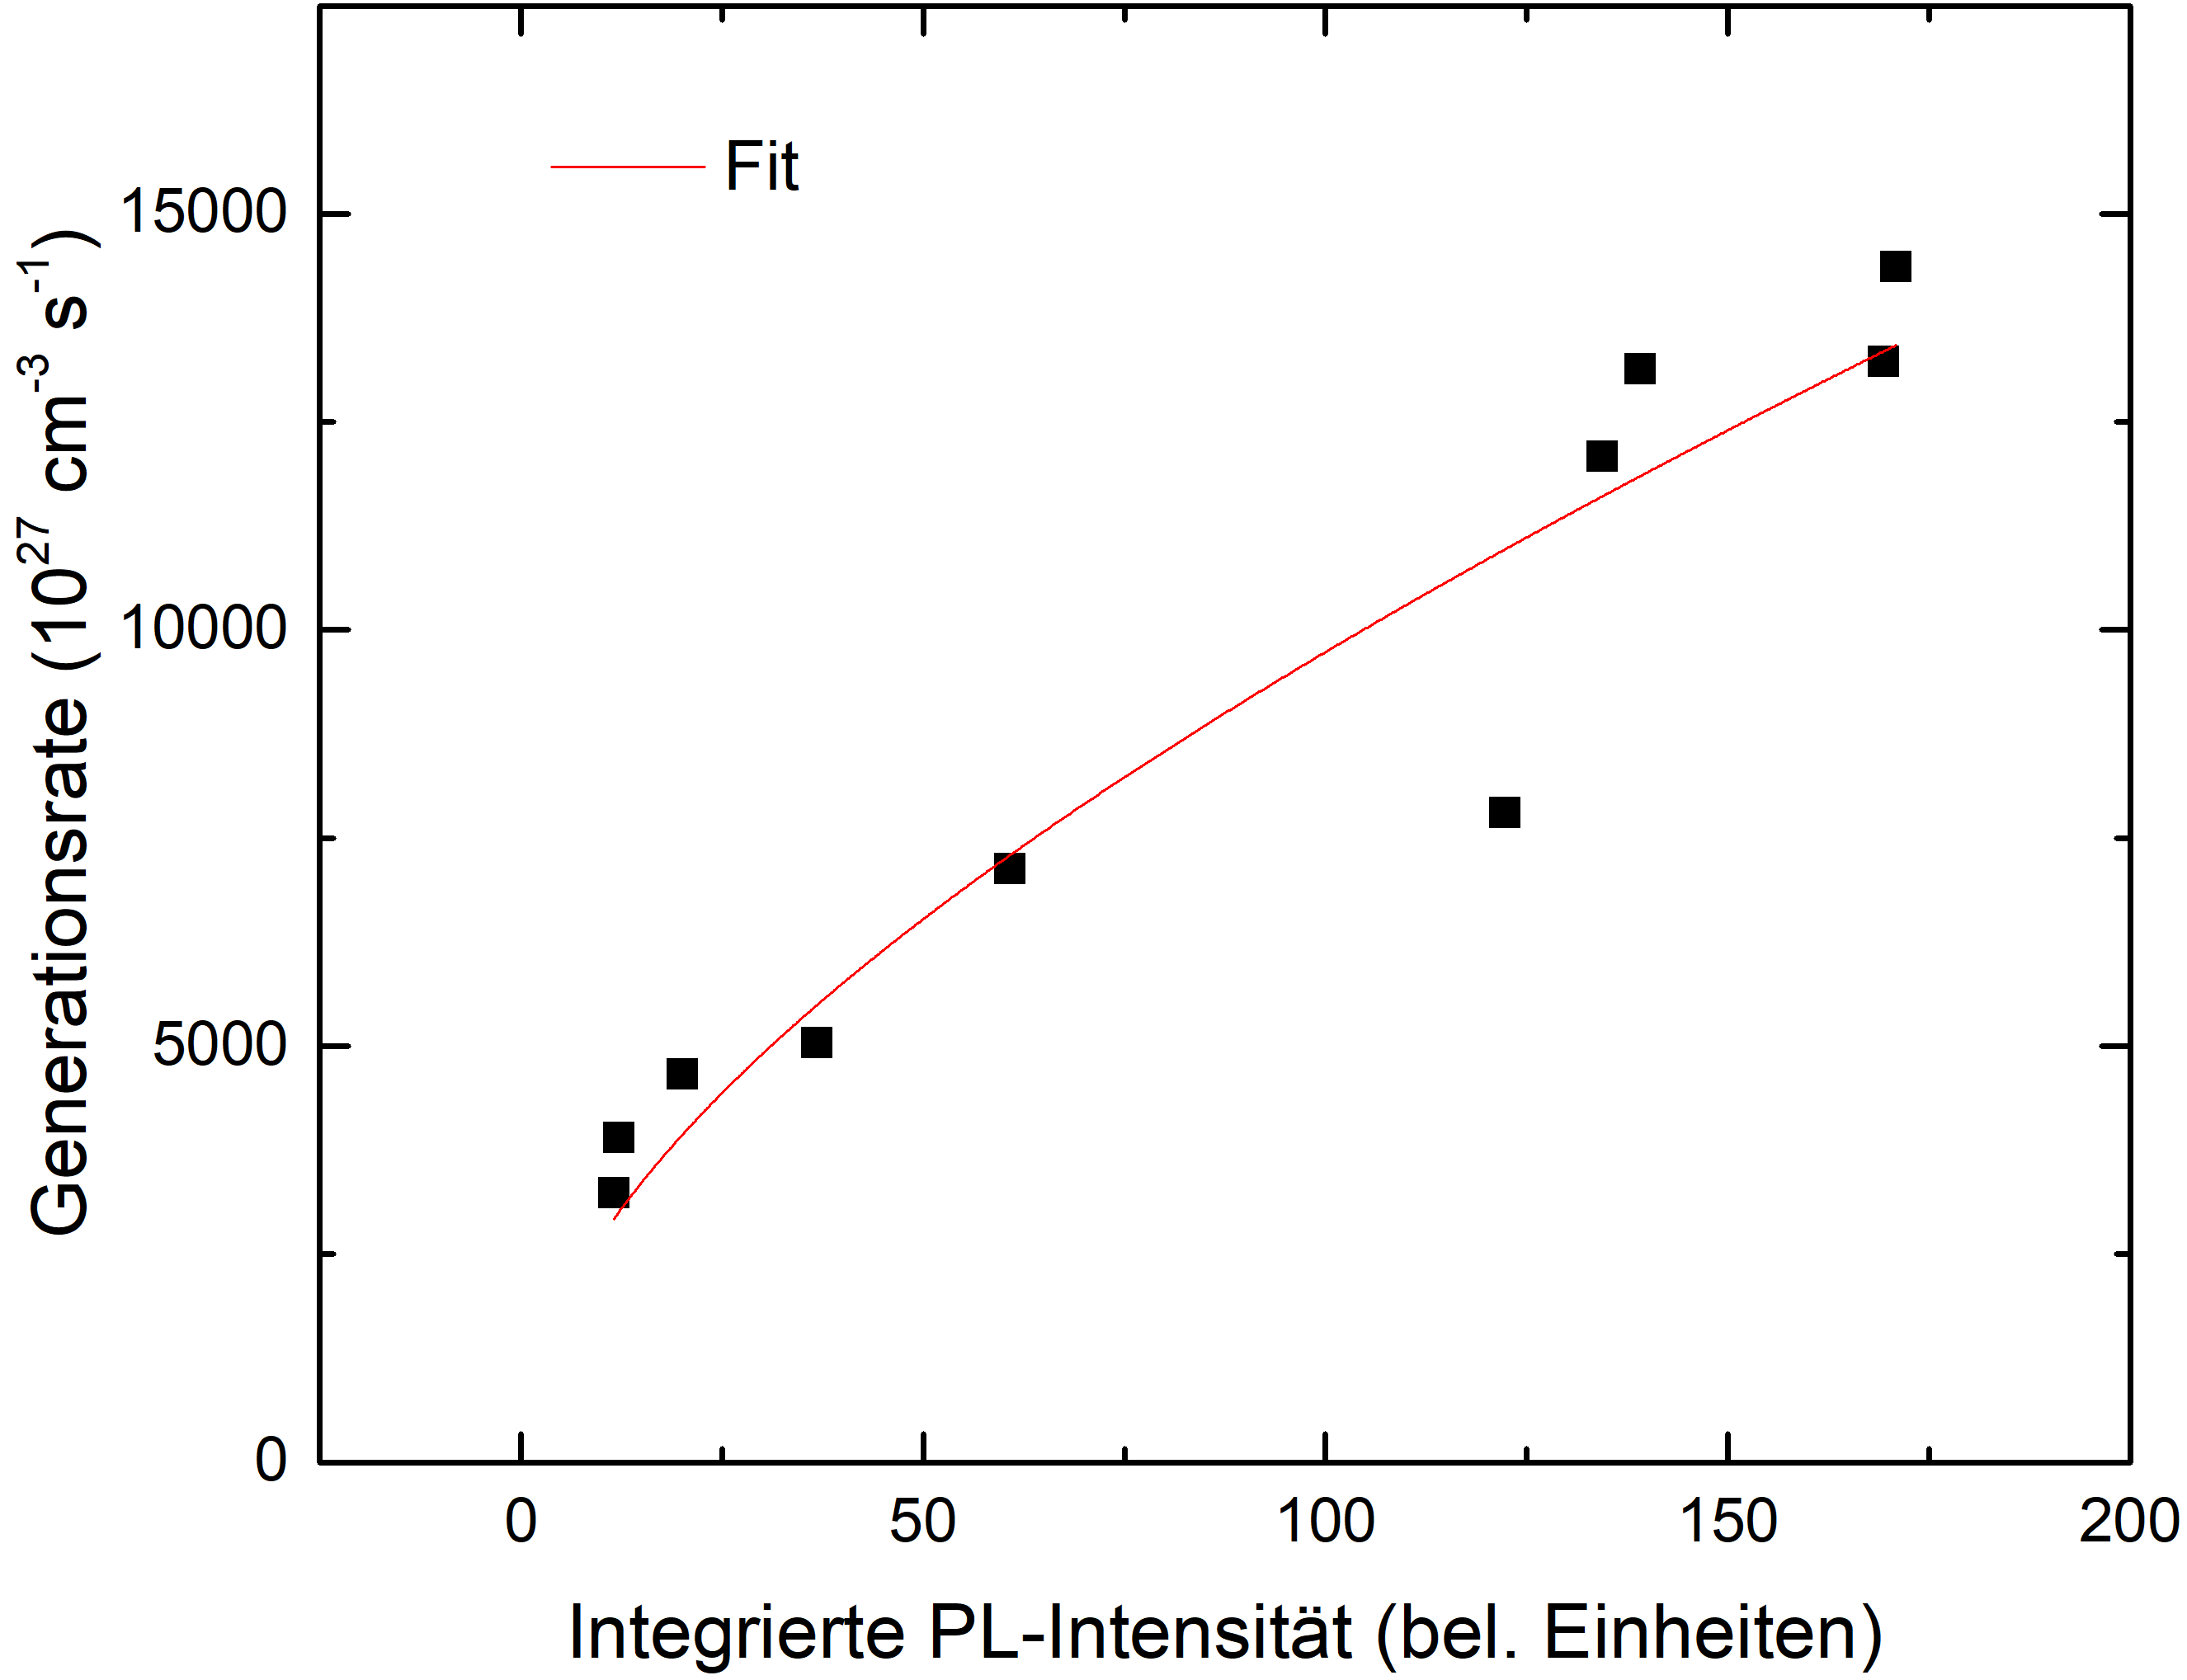
\includegraphics[width=0.30\textwidth]{Bilder/RaumtempBilder/genfit1-10.png} & 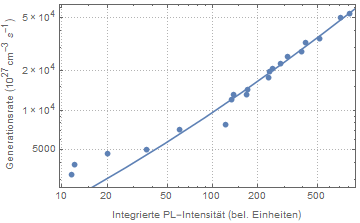
\includegraphics[width=0.30\textwidth]{Bilder/RaumtempBilder/genfit1-20.png}  & 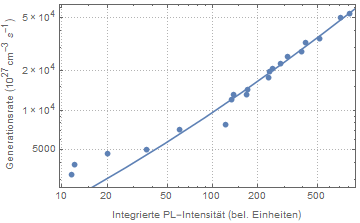
\includegraphics[width=0.30\textwidth]{Bilder/RaumtempBilder/genfit1-20.png} \\
 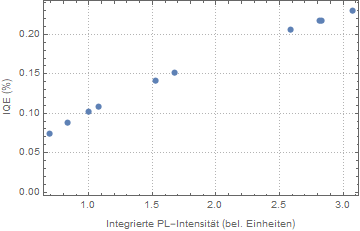
\includegraphics[width=0.30\textwidth]{Bilder/RaumtempBilder/iqe1-10.png} &   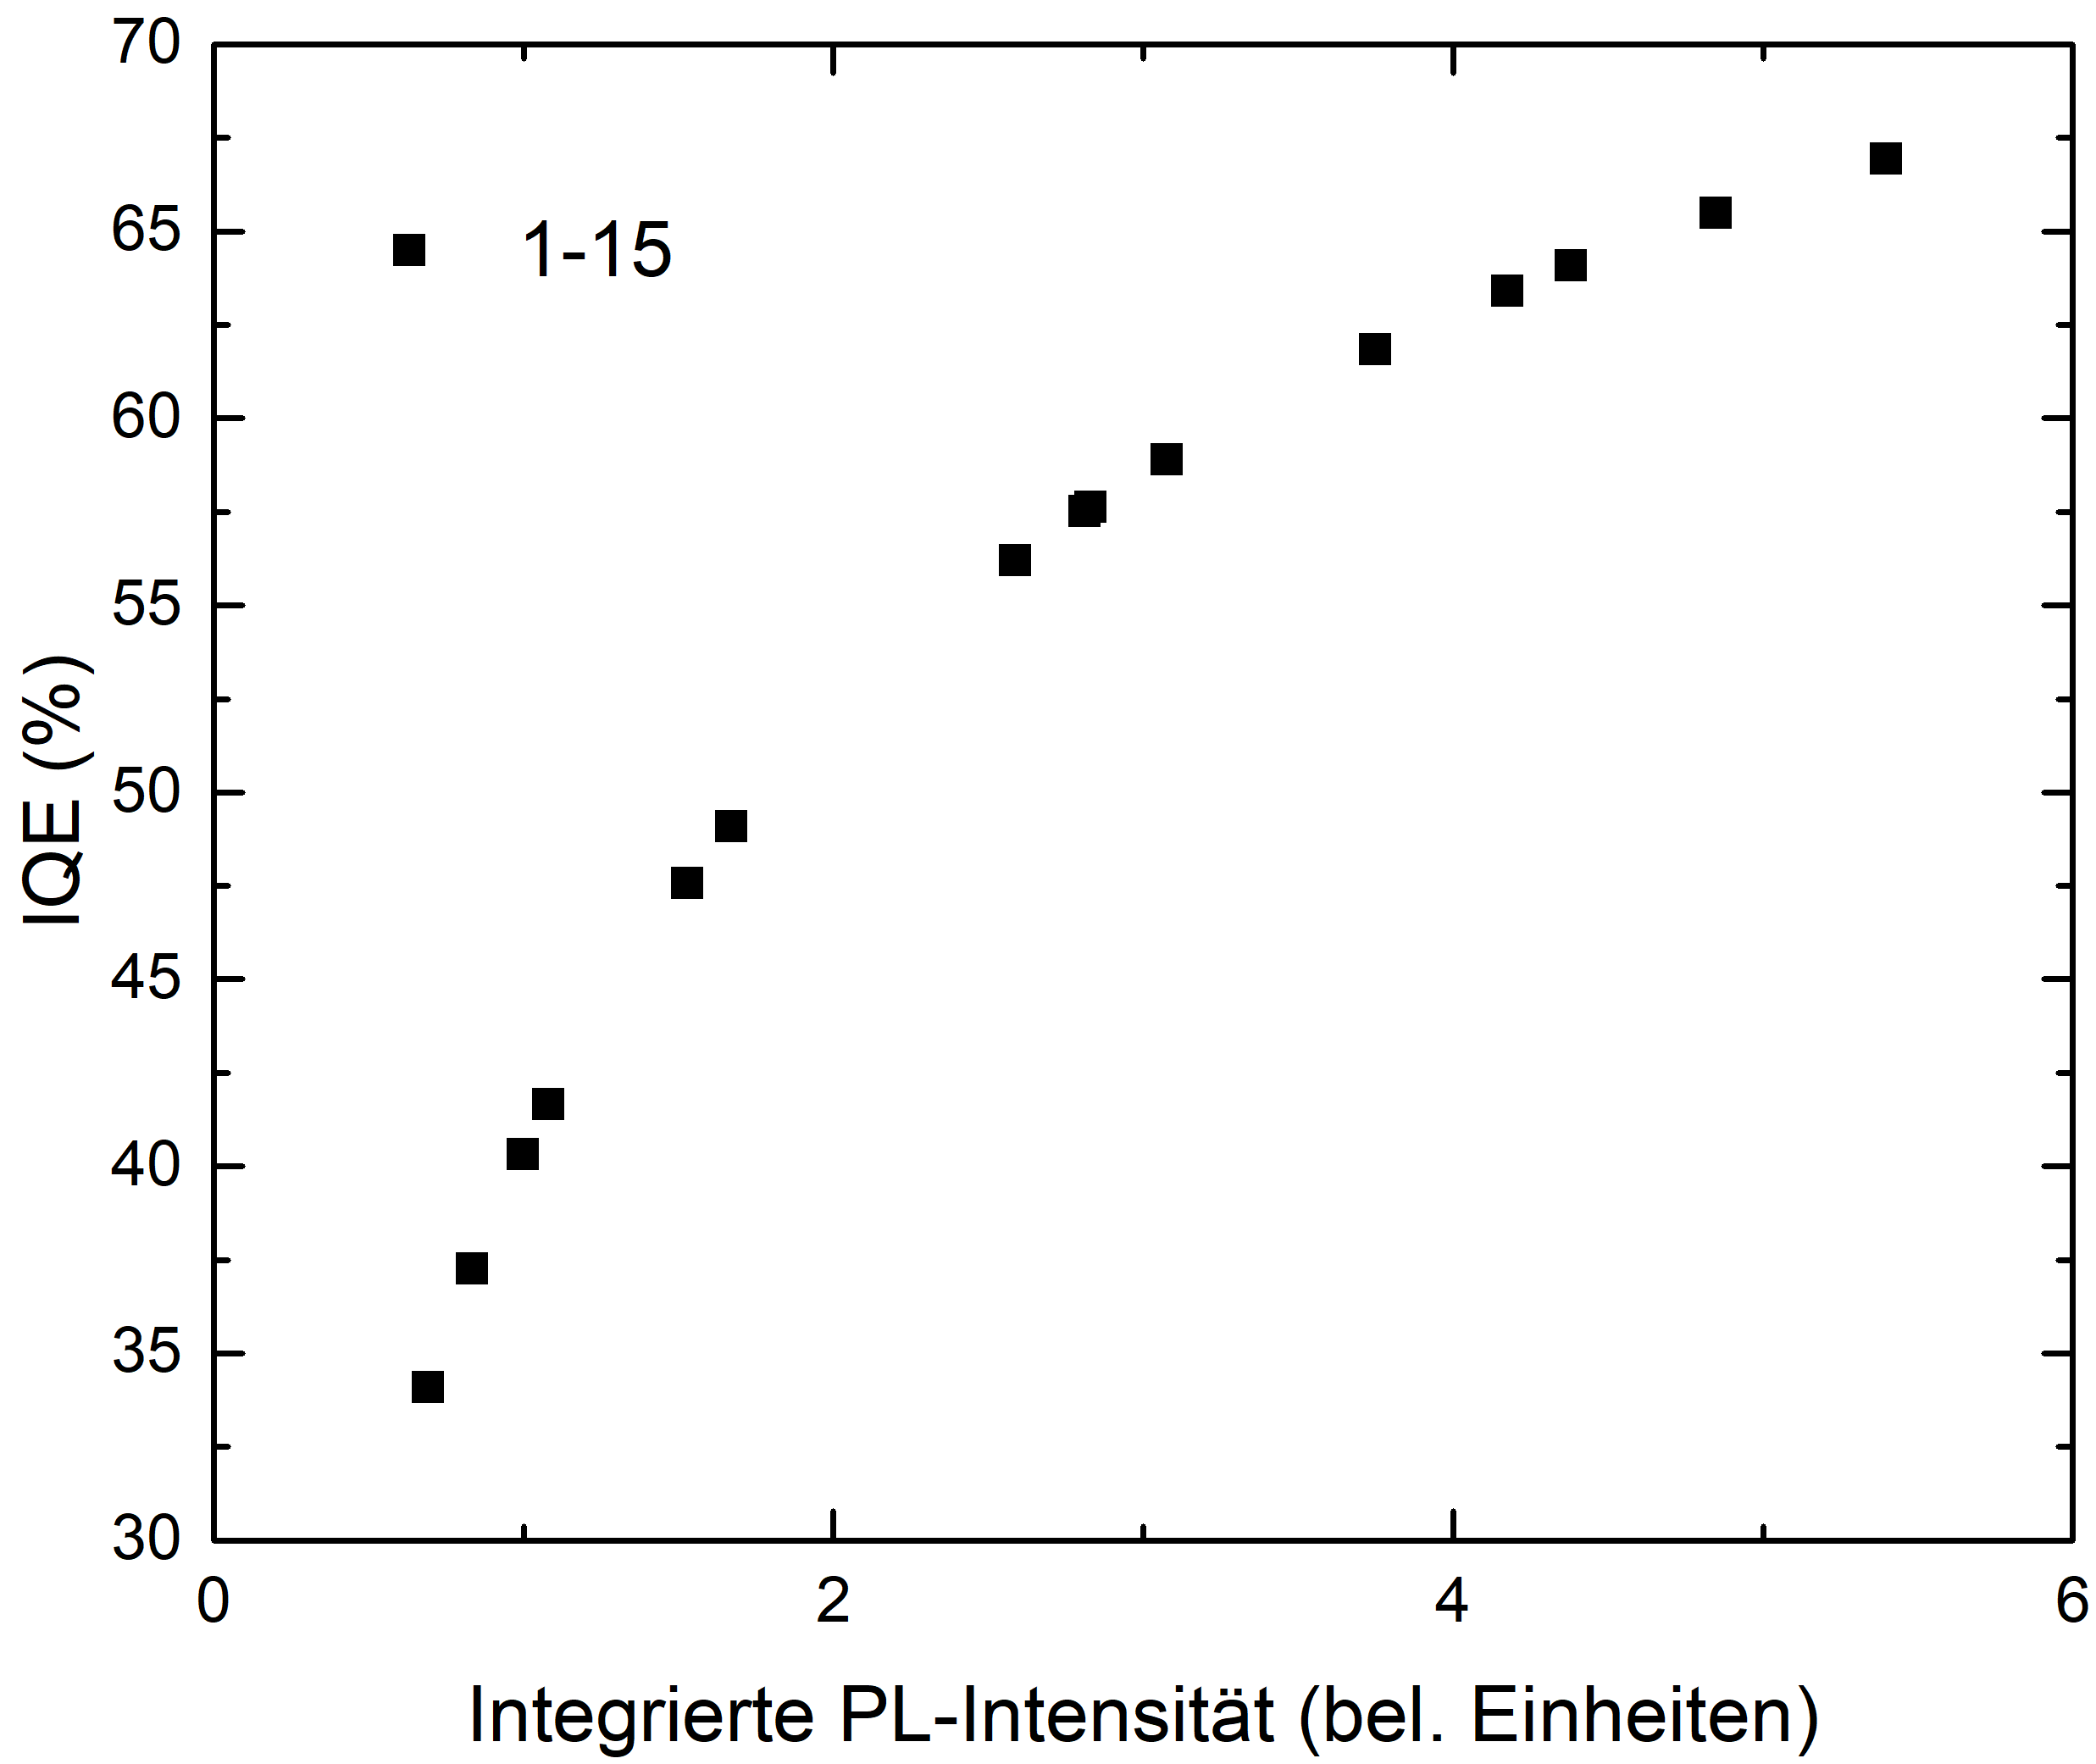
\includegraphics[width=0.30\textwidth]{Bilder/RaumtempBilder/iqe1-15.png} & 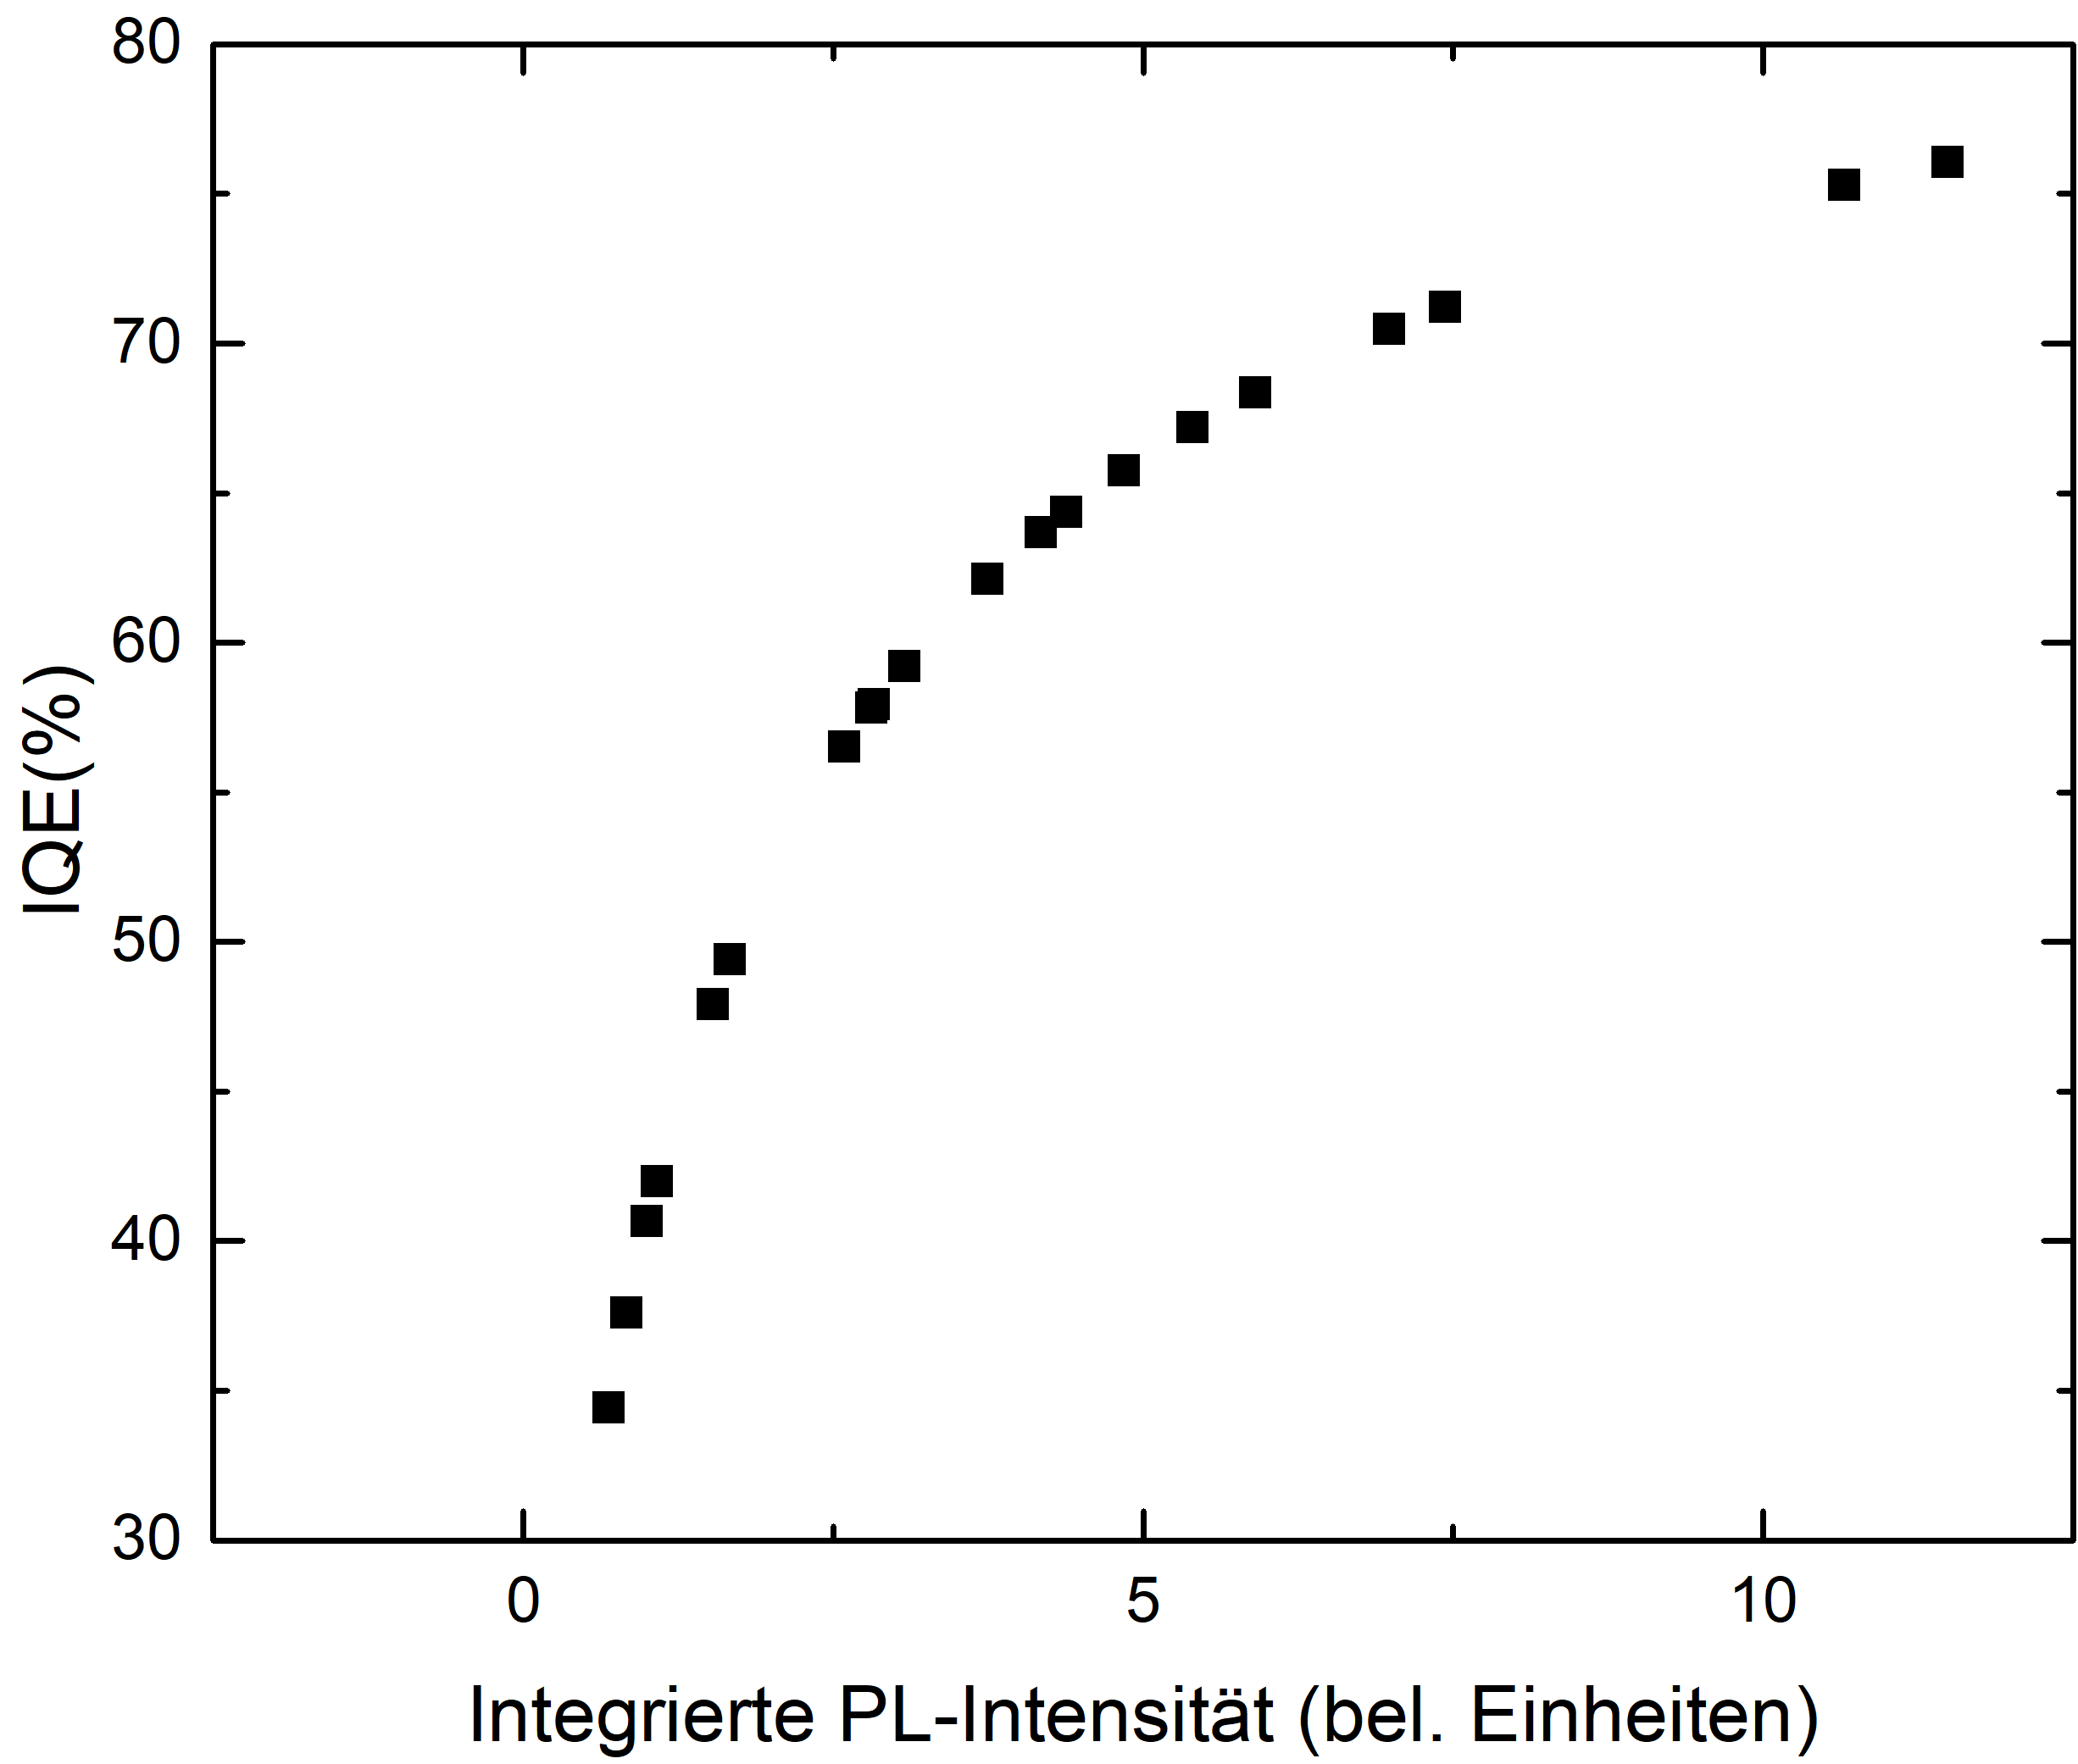
\includegraphics[width=0.30\textwidth]{Bilder/RaumtempBilder/iqe1-20.png}  \\
 a & b & c
\end{tabular}
\caption{Der Fit der Generationsrate in Abhängigkeit der integrierten Intensität für die 1-5 (a), 1-10 (b) und 1-15 (c) Datenpunkte und darunter die aus dem Fit bestimmte IQE.}
\label{fig:raumtemp}
\end{figure}
\noindent 
Abbildung \ref{fig:raumtemp} zeigt exemplarisch die Abhängigkeit der resultierenden IQE aus den ausgewählten Datenpunkten.
Dies wiederholt sich, so dass die Methode für keine Probenserie verlässliche IQE Werte liefert und stattdessen die Ergebnisse mit dem ausgewählten Bereich der Datenpunkte immer stark variieren.
\newline
Des Weiteren waren die zugehörigen A- und B-Parameter nicht im Größenordnungsbereich der Literaturwerte, die in Kapitel \ref{chap:rekomb} angegeben sind. Stattdessen schwanken sie variierend mit einigen Zehnerpotenzen darüber oder darunter in Abhängigkeit des ausgewählten Bereiches.
\newline
Weshalb das Modell keine verlässlichen Resultate liefert, hat mehrere Gründe. 
Die Methode setzt voraus, dass die Auger-Rekombination vernachlässigt werden kann, da nur Bereiche geringer Anregungsleistungsdichte betrachtet werden sollen. Dieser Bereich leidet aber insbesondere bei Raumtemperatur an starkem Rauschen. 
\newline
Zusätzlich betrachtet die Methode den möglichen Einfluss einer Dotierung überhaupt nicht. Dies ist, wie in Kapitel \ref{chap:mqw} gezeigt wird, nicht zu vernachlässigen.
\newline
Ein weiterer wichtiger Punkt ist, dass mit dem verwendeten Setup (Kapitel \ref{chap:aufbau}) keine Möglichkeit besteht, nur die QWs anzuregen und so der Effekt der thermischen Diffusion  deutlichen Einfluss nimmt. Dies wird jedoch ebenfalls nicht vom Modell berücksichtigt und führt in Kombination mit den erwähnten anderen Gründen dazu, dass die Anwendung der Methode scheitert.
\newline
%Bei Proben mit Laserstruktur (erste und letzte Barriere des MQWs sind Waveguides) fiel insbesondere auf, dass die Form der Kurve von der des Fits besonders stark abweicht und wahrscheinlich bedingt ist, durch die komplexere Struktur im Vergleich zu normalen LED-Strukturen. 

